In this section, we'll begin combining the basic elements---operators
and states---covered in previous sections.
As discussed in the introduction, our methods of combination
correspond to \emph{space}, \emph{time},  and \emph{function}, in ways
we are about to make process. Roughly speaking, tensor products
compose systems in spatial parallel; conjugation uses an operator to
evolve an observable or state; and finally, channels generalize
both conjugation and measurement, randomly evolving states and
observables with a well-behaved set of operators.

\subsection*{Conjugation}

Conjugation is familiar from Heisenberg evolution of operators and
change of basis in linear algebra. For a
time evolution operator $U$, an observer $A$ evolves as
\[
  A \mapsto U^* A U = U \triangleright A.
\]
Thinking of the functional $\pi(\cdot)$ as the expectation $\langle
\pi | \cdot |\pi\rangle$, the Heisenberg evolution corresponds to
Schr\"{o}dinger evolution
\[
  \langle
\pi | A |\pi\rangle \mapsto \langle
\pi | U^* A U|\pi\rangle = \pi(U \triangleright A) = [U \triangleleft \pi](A).
\]
The infix operators $\triangleright, \triangleleft$ are a little
slicker than conventional alternatives,\sidenote{The ``adjoint
  action'' notation $\text{Ad}_U$ and its pullback $\text{Ad}_U^*$.}
and in \texttt{yaw}, they are implemented by \texttt{»},
\texttt{«}.\sidenote{On Mac OS, \texttt{»} = \texttt{Option} +
  $\mathtt{\backslash}$ and \texttt{«} = \texttt{Shift} +
  \texttt{Option} + $\mathtt{\backslash}$. You can also simply type
  \texttt{>}\texttt{>} and \texttt{<}\texttt{<}.} For instance, conjugating $X$ by the Hadamard gate $H = (X
+ Z)/\sqrt{2}$ yields $Z$, and vice-versa, and simply adds a phase to $Y$:
\begin{minted}
     [
frame=lines,
framesep=2mm,
baselinestretch=1.2,
bgcolor=AliceBlue,
fontsize=\footnotesize,
linenos
]{slurm}
    *> H = (X + Z)/sqrt(2)
    *> H » X
    Z
    *> H » Z
    X
    *> H » Y
    -1j*X*Z
\end{minted}
Similarly, state conjugation swaps eigenfunctionals of $X$ and
$Z$:
\begin{minted}
     [
frame=lines,
framesep=2mm,
baselinestretch=1.2,
bgcolor=AliceBlue,
fontsize=\footnotesize,
linenos
]{slurm}
    *> Z | H « char(X,0)
    1
    *> X | H « char(Z,0)
    1
\end{minted}

In the usual ``Schr\"{o}dinger picture'', we take an input state
$|\pi\rangle$, evolve by a unitary $|\pi\rangle \mapsto U|\pi\rangle$, and measure. In our algebraic
``Heisenberg picture'', we take an input state $\pi$, conjugate by a
unitary $\pi \mapsto U \triangleleft \pi$, and measure. (We explain
the mmeasurement step below.) The result of two circuits,
$|\pi\rangle \mapsto U_2 (U_1 |\pi\rangle)$ becomes $\pi \mapsto U_2
\triangleleft (U_1 \triangleleft \pi)$. This is different from
\[
  \pi \mapsto (U_2 \triangleright U_1) \triangleleft \pi = (U_2^* U_1 U_2) \triangleleft \pi,
\]
which is an important design pattern in quantum algorithms.
Many quantum algorithms take the form \marginnote{
  \vspace{-80pt}
  \begin{center}
    \hspace{-10pt}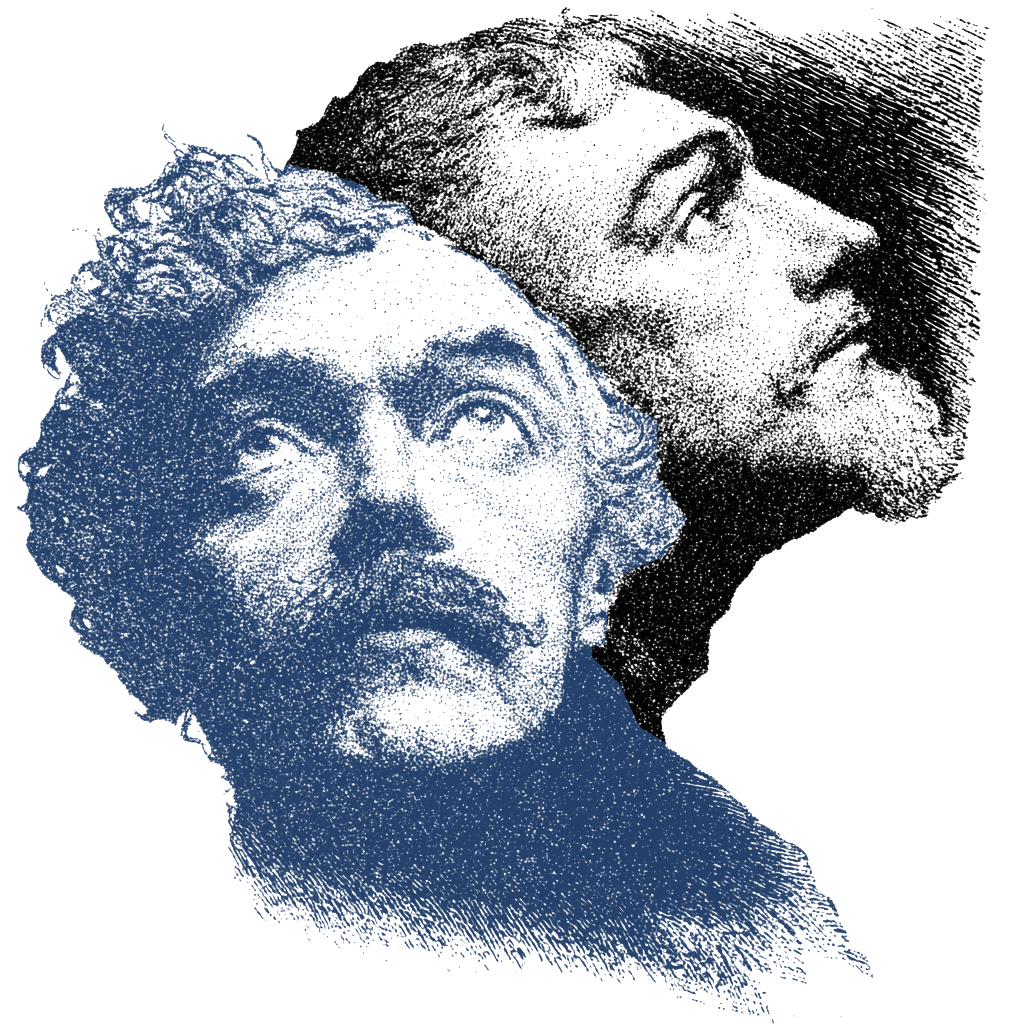
\includegraphics[width=0.95\linewidth]{img/double}
  \end{center}  \vspace{-5pt}
  \emph{The QFT is a change of perspective.
  } \vspace{-10pt}
}
\[
  \pi \mapsto (\text{QFT} \triangleright U) \triangleleft \pi
\]
for the \emph{quantum Fourier transform} $\text{QFT}$ which,
generalizing the Hadamard $H$,  exchanges $Z$ for the $X$ operator
(and the $X$ operator for $Z^{d-1}$) in the
generalized Clifford algebra $\mathcal{A}_d$.
This is invoked via \texttt{qft(X, Z)}, though you can formally
exchange other operators as well:
\begin{minted}
     [
frame=lines,
framesep=2mm,
baselinestretch=1.2,
bgcolor=AliceBlue,
fontsize=\footnotesize,
linenos
]{slurm}
    *> $alg = qudit(d)
    *> W1 = qft(X, Z)
    *> W1 » Z
    X
    *> W1 » X
    X**(d-1)
    *> W2 = qft(X, Y)
    *> W2 » Y
    X
\end{minted}
% Here, \texttt{d} is a parameter of your choice.
The initial $\text{QFT} \triangleleft \pi$ step in the $(\text{QFT}
\triangleright U) \triangleleft \pi$ pattern often just changes an
eigenfunctional $\pi^{(Z)}_0$ for an eigenfunctional $\pi^{(X)}_0$.
% In some cases it's simpler to just start in a different state.
Sometimes, it's simpler to start in the right place.

\subsection*{Tensor products}

When you have two systems governed by algebras $\mathcal{A}_1$ and
$\mathcal{A}_2$, the joint system is described by a tensor product
$\mathcal{A}_1\otimes \mathcal{A}_2$. Operators on the joint system
take the form of (limits of) terms of the form
\[
  \sum_{i=1}^N c_i A_{1,i} \otimes A_{2,i}, \quad \text{for} \, A_{1,i} \in \mathcal{A}_1, A_{2,i} \in \mathcal{A}_2.
\]
We can build states on the tensor product from tensor products of
states, with $S(\mathcal{A}_1)\otimes S(\mathcal{A}_2) \subseteq
S(\mathcal{A}_1\otimes \mathcal{A}_2)$ since we can define
\[
 (\pi_1\otimes\pi_2)(A_1 \otimes A_2) = \pi_1(A_1)\pi_2(A_2).
  \]
  However, entanglement means that not every state has this form. For
  instance, we will construct the \emph{EPR state} below, with
  \begin{equation}
    \pi(A) = \frac{1}{2}(\langle 00| + \langle 11|) A (|00\rangle +
    |11\rangle).\label{eq:epr}
  \end{equation}
  There is no way to factorize this, as you can show in Exercise 3.2.
%   \[
% S(\mathcal{A}_1)\otimes S(\mathcal{A}_2) \subsetneq  S(\mathcal{A}_1\otimes \mathcal{A}_2).
% \]
% As a simple example, for two qubits, $\pi^{(Z)}_0 \otimes
% \pi^{(Z)}_{0}$ is a valid state, but there are states that cannot be
% written in the product form $\pi_1 \otimes \pi_2$ for any $\pi_1,
% \pi_2$.
%We'll construct an example shortly!
% so we can build states on $\mathcal{A}_1\otimes \mathcal{A}_2$
% from sums of products of a state on $\mathcal{A}_1$ and a state on
% $\mathcal{A}_2$.
\newpage

In \texttt{yaw}, working with tensor products is simple.
First, we can automatically build tensor products from the global
algebra using the \texttt{@} infix and tensor powers using the \texttt{(@n)} prefix:
\begin{minted}
     [
frame=lines,
framesep=2mm,
baselinestretch=1.2,
bgcolor=AliceBlue,
fontsize=\footnotesize,
linenos
]{slurm}
    *> $alg = qubit()
    *> XXX = X @ X @ X
    *> ZZZ = (@3) Z
    *> XXX*ZZZ
    X*Z @ X*Z @ X*Z
    *> psi3 = (@3) char(Z, 0)
    *> ZZZ | psi3
    1
\end{minted}
You can also refer to different algebras, and operators therein, using
the \texttt{alg.op} notation, and explicitly build the QFT over
different algebras with \texttt{tensor\_qft}:
\begin{minted}
     [
frame=lines,
framesep=2mm,
baselinestretch=1.2,
bgcolor=AliceBlue,
fontsize=\footnotesize,
linenos
]{slurm}
    *> alg1 = qudit(3)
    *> alg2 = qudit(5)
    *> qft1 = qft(alg1.X, alg1.Z)
    *> qft2 = qft(alg2.X, alg2.Z)
    *> W = tensor_qft(qft1, qft2)
\end{minted}
Finally, conjugation works as expected:
\begin{minted}
     [
frame=lines,
framesep=2mm,
baselinestretch=1.2,
bgcolor=AliceBlue,
fontsize=\footnotesize,
linenos
]{slurm}
    *> W » alg1.Z @ alg2.Z
    alg1.X @ alg2.X
\end{minted}
Note that operators in the global \texttt{\$alg} are unlabelled,
but otherwise distinguished by the algebra object they belong to.

Let's see how this works in practice and build an entangling operator.
The controlled-$X$ or CNOT${}_d$ is an operator on two qudits which applies
$X^k$ on the second qudit when the first is in state
$\pi^{(Z)}_k$. Accordingly, we introduce projectors $\Pi^{(Z)}_k$ to
sift out the states $\pi^{(Z)}_k$ on the first qudit, with $X^k$ on the second:
\begin{equation}
  \text{CNOT}_d = \sum_{k=0}^{d-1}\Pi^{(Z)}_k \otimes X^k.\label{eq:8}
\end{equation}
Let's implement it in full generality:
% \sidenote{As usual, you must
%   pick \texttt{d} for this code to work.}
\begin{minted}
     [
frame=lines,
framesep=2mm,
baselinestretch=1.2,
bgcolor=AliceBlue,
fontsize=\footnotesize,
linenos
]{slurm}
    *> $alg = qudit(d)
    *> CNOT = sum(proj(Z,k) @ X**k for k in range(d))
\end{minted}
The ordinary $\text{CNOT}$ is the special case of $d=2$.
We can check it behaves as intended by acting on functional
$\pi^{(X)}_0\otimes \pi^{(Z)}_0$, which corresponds to a vector
\[
  |+\rangle |0\rangle = \frac{1}{\sqrt{2}} (|00\rangle + |10\rangle)
  \overset{\text{CNOT}}{\longmapsto} \frac{1}{\sqrt{2}} (|00\rangle + |11\rangle),
\]
where the latter is called the EPR state:
\begin{minted}
     [
frame=lines,
framesep=2mm,
baselinestretch=1.2,
bgcolor=AliceBlue,
fontsize=\footnotesize,
linenos
]{slurm}
    *> init = char(X, 0) @ char(Z, 0)
    *> EPR = CNOT « init
\end{minted}
This state is characterized by the fact that, when we restrict to the
first or the second qubit, the state is \emph{completely mixed},
meaning its expectations for $X$, $Y$ and $Z$ are the same as if we
averaged over all states. By symmetry, this means they
vanish.\sidenote{The fact that $\text{spec}(X) = \{\pm1\}$ implies the symmetry
  $X \mapsto -X$, and so on.} Let's check:
\begin{minted}
     [
frame=lines,
framesep=2mm,
baselinestretch=1.2,
bgcolor=AliceBlue,
fontsize=\footnotesize,
linenos
]{slurm}
    *> [op | EPR for op in [X @ I, Y @ I, Z @ I]]
    [0.0, 0.0, 0.0]
    *> [op | EPR for op in [I @ X, I @ Y, I @ Z]]
    [0.0, 0.0, 0.0]
\end{minted}
Note that \texttt{X @ I} is a partial measurement of $X$ on the first
qubit, and so forth. You can explore the qudit version in Exercise 3.2. % \marginnote{
%   \vspace{-80pt}
%   \begin{center}
%     \hspace{-10pt}\includegraphics[width=0.95\linewidth]{img/ghosts}
%   \end{center}  \vspace{-5pt}
%   \emph{Spooky action.
%   } \vspace{-10pt}
% }
On the other hand, joint measurements of the same operator are always
perfectly correlated:
\begin{minted}
     [
frame=lines,
framesep=2mm,
baselinestretch=1.2,
bgcolor=AliceBlue,
fontsize=\footnotesize,
linenos
]{slurm}
    *> [op | EPR for op in [X @ X, Y @ Y, Z @ Z]]
    [1, -1, 1]
\end{minted}
To check this ``spooky'' correlation more explicitly, we need to
introduce the machinery of measurement and channels.

\subsection*{Channels and measurement}

A \emph{channel} is a sum of conjugators that maps the identity to itself:
\begin{equation}
  \label{eq:9}
  \mathcal{C}_{\mathfrak{L}} = \sum_{\lambda\in \mathfrak{L}}
  K_\lambda\, \triangleright, \quad   \mathcal{C}_{\mathfrak{L}}[I] = \sum_{\lambda\in \mathfrak{L}}
  K_\lambda^*  K_\lambda = I.
\end{equation}
The operators $B_k$ are called \emph{Kraus operators}.
The dual \emph{state channel} is the corresponding sum of state conjugators,
and dual to the property of preserving the identity (called
``unitality'') is the property of preserved \emph{trace}:\sidenote{In the
situations this is defined, e.g. density matrices on a
finite-dimensional GNS space. The proof here uses linearity and
cyclicity of the trace, $\mbox{tr}[AB]=\mbox{tr}[BA]$.}
\begin{equation}
  \label{eq:9}
  \mathcal{C}^{\mathfrak{L}} = \sum_{\lambda\in \mathfrak{L}}
  K_\lambda\, \triangleleft, \quad   \mbox{tr}\,\mathcal{C}^{\mathfrak{L}}[\pi] = \sum_{\lambda\in \mathfrak{L}}
\mbox{tr}\big[ K_\lambda\pi  K_\lambda^* \big] = \mbox{tr}[\pi].
\end{equation}
The channel can simply be applied, as in the case of errors.
The \emph{depolarizing channel} $\Delta_\alpha$, usually written in
the state form, mixes a qubit state with the maximally mixed state
$I/2$:\sidenote{Again, this is in the setting of density matrices on a
finite-dimensional GNS space.}
\[
  \Delta_\alpha[\pi] = (1-\alpha)\pi + \frac{\alpha}{2} I.
\]
As you can show in Exercise 3.3, this has Kraus operators
\[
  B_0 =\sqrt{1 - \frac{3\alpha}{4}} I, \quad B_i = \sqrt{\frac{\alpha}{4}}\sigma_i,
\]
where we recall that $\sigma_1 = X$, $\sigma_2 = Y$ and $\sigma_3 = Z$.

We can define the state channel easily in \texttt{yaw} using
\texttt{stChannel}:
\begin{minted}
     [
frame=lines,
framesep=2mm,
baselinestretch=1.2,
bgcolor=AliceBlue,
fontsize=\footnotesize,
linenos
]{slurm}
    *> $alg = qubit()
    *> sigma = [X, 1j*X*Z, Z]
    *> def stDpl(alpha):
    ...    K0 = sqrt(1-3*alpha/4)*I
    ...    Ks = [sqrt(alpha/4)*sigma[i] for i in range(3)]
    ...    return stChannel([K0]+Ks)
    *> dplZ = stDpl(0.2)(char(Z,0))
    *> Z | dplZ
    0.8
\end{minted}
We can also compute the effect of the channel on operators directly
with \texttt{opChannel}:
\begin{minted}
     [
frame=lines,
framesep=2mm,
baselinestretch=1.2,
bgcolor=AliceBlue,
fontsize=\footnotesize,
linenos
]{slurm}
    *> def opDpl(alpha):
    ...    K0 = sqrt(1-3*alpha/4)*I
    ...    Ks = [sqrt(alpha/4)*sigma[i] for i in range(3)]
    ...    return opChannel([K0]+Ks)
    *> opDpl(0.2)(Z)
    *> 0.8*Z
\end{minted}
By analogy with \texttt{Unix}, pipe syntax allows us to push operators
through a chain of channels, and optionally, to evaluate in a
state at the end:
\begin{minted}
     [
frame=lines,
framesep=2mm,
baselinestretch=1.2,
bgcolor=AliceBlue,
fontsize=\footnotesize,
linenos
]{slurm}
    *> Z | opDpl(0.2) | opDpl(0.8) | stDpl(0.4)(char(Z, 0))
    *> 0.096
\end{minted}
The final state evaluation is in fact another form of operator
channel,\sidenote{Albeit one that sends operators to complex numbers.} so our
notation is consistent.

So far, we've treated channels as black boxes that process inputs
undisturbed. But we can open up and look inside! This is the act of
measurement, and %it disturbs the processing in such a way that only
it effectively chooses a Kraus operator at random
\begin{equation}
  A \overset{\text{evolve}}{\longmapsto} \mathcal{C}_{\mathfrak{L}}[A] = \sum_{\lambda\in
    \mathfrak{L}} K_\lambda^*A K_\lambda
  \overset{\text{observe}}{\longmapsto} \frac{1}{C_\lambda}
  K_\lambda^*A K_\lambda,\label{eq:opMeasure}
\end{equation}
according to the \emph{L\"{u}ders rule}. Similarly:
\begin{equation}
    \pi \overset{\text{evolve}}{\longmapsto} \mathcal{C}^{\mathfrak{L}}[\pi] = \sum_{\lambda\in
    \mathfrak{L}} K_\lambda \triangleleft \pi
  \overset{\text{observe}}{\longmapsto} \frac{1}{C_\lambda} (K_\lambda
  \triangleleft \pi).\label{eq:stMeasure}
\end{equation}
Here, $C_\lambda$ is a normalization constant that depends on the state
$\pi$ we observe in; to ensure the output state remains
normalized, we have\sidenote{This follows from \[C_\lambda^{-1} (K_\lambda \triangleleft
    \pi)(I) = C_\lambda^{-1} \pi (K_\lambda^* K_\lambda) = 1.\]} %it can only take the value
\begin{equation}
  \label{eq:10}
 C_\lambda = \pi (K_\lambda^* K_\lambda).
\end{equation}
The fact that the operator channel is unital, i.e. maps $I$ to itself,
means that the constants sum to unity:\marginnote{
  \vspace{-80pt}
  \begin{center}
    \hspace{-10pt}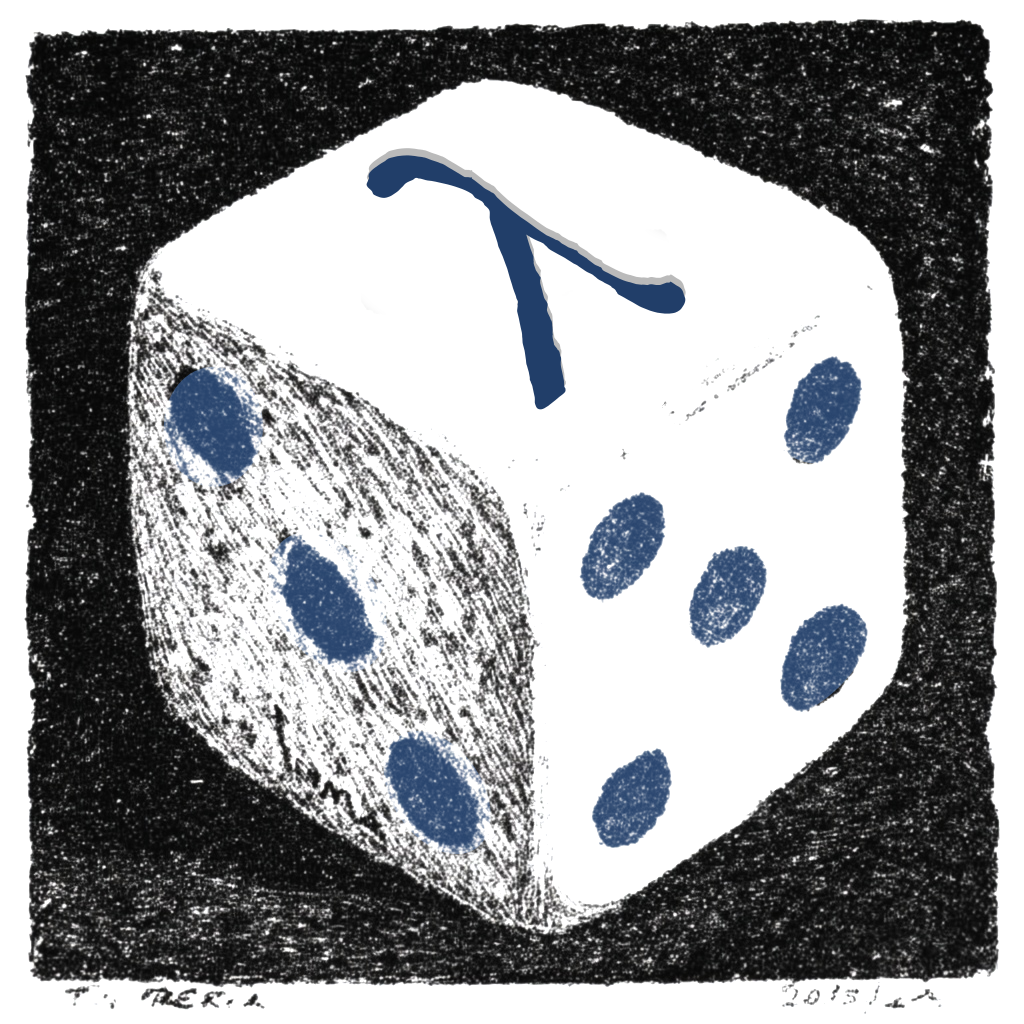
\includegraphics[width=0.95\linewidth]{img/lambda}
  \end{center}  \vspace{-5pt}
  \emph{Observing a channel is a roll of the Kraus.
  } \vspace{-10pt}
}
\[
  \sum_{\lambda\in\mathfrak{L}} C_\lambda = \pi
  \left(\sum_{\lambda\in\mathfrak{L}} K_\lambda^* K_\lambda\right) =
  \pi(I) = 1,
\]
with positivity implying that each $C_\lambda \geq 0$. This looks a
lot like probability, and indeed, \emph{Born's rule} tells us that $C_\lambda$
is the probability of observing Kraus operator $\lambda$.

In \texttt{yaw}, measurement can either be performed with respect to
operators (\ref{eq:opMeasure}) via \texttt{opMeasure}, or states
(\ref{eq:stMeasure}) via \texttt{stMeasure}. We can illustrate with
the $Z$-measurement of a qubit in the $\pi^{(X)}_0$ state:
\begin{minted}
     [
frame=lines,
framesep=2mm,
baselinestretch=1.2,
bgcolor=AliceBlue,
fontsize=\footnotesize,
linenos
]{slurm}
    *> Ks = [proj(Z, 0), proj(Z, 1)]
    *> psi = char(X, 0)
    *> psiNew, outcome = stMeasure(Ks, psi)()
    *> outcome
    1
    *> Z | psiNew
    -1
\end{minted}
The function \texttt{opMeasure} works in a similar way. A useful
shortcut when the Kraus operators are projectors of some observable is
given by the simpler \texttt{measure} function:
\begin{minted}
     [
frame=lines,
framesep=2mm,
baselinestretch=1.2,
bgcolor=AliceBlue,
fontsize=\footnotesize,
linenos
]{slurm}
    *> psiNew, outcome = measure(Z, psi)()
\end{minted}
%This decomposes the observable for us!
We can now revisit the entanglement example:
\begin{minted}
     [
frame=lines,
framesep=2mm,
baselinestretch=1.2,
bgcolor=AliceBlue,
fontsize=\footnotesize,
linenos
]{slurm}
    *> init = char(X, 0) @ char(Z, 0)
    *> EPR = CNOT « init
    *> [measure(X@X, EPR)()[1] for _ in range(10)]
    [0, 0, 0, 0, 0, 0, 0, 0, 0, 0]
    *> [measure(Z@Z, EPR)()[1] for _ in range(10)]
    [0, 0, 0, 0, 0, 0, 0, 0, 0, 0]
    *> [measure(X@Z, EPR)()[1] for _ in range(10)]
    [1, 1, 1, 0, 0, 1, 0, 1, 1, 1]
\end{minted}
Every time we measure the same observable on both qubits, we get the
same answer; different observables get different answers.\sidenote{If
  we get outcomes $a, b \in \{0, 1\}$, we return the sum $a \oplus b$
  modulo $2$. %, which vanishes just in case $a = b$. See the
  % exercises for moredetails.
} 

\newpage

% We end with a slightly different perspective on measurement. For
% understanding algorithms, it can be useful to keep track of the
% different ``branches'' of the wavefunction

\subsection*{Coda}
\label{sec:coda}

We've now seen three elementary ways to compose quantum algorithms:
conjugation, tensor products, and channels. Indeed, these are the three
basic combinators in the standard approach to quantum computing, which
takes a ficidual initial states $|0^n\rangle$ over multipe qubits
(tensor product), evolves by a circuit $|0^n\rangle\mapsto U
|0^n\rangle$ (conjugation), and finally measures in a fixed basis
(channels). We have given the toy example of building and measuring an
entangled state, but although simple, it hopefully begins to hint at
the elegance and power of the algebraic approach. To make those hints
fully manifest, however, we need to start thinking about real algorithms.